%----------------------------------------------------------------------------
\chapter{Experiments and results}\label{sect:Experiments}
%----------------------------------------------------------------------------

In this chapter I will present my results achieved on the data. The two classes (whether to include a word or edge in the summary) appear disproportionally in the dataset. There is 2.5 times more node that we leave out from the summaries then nodes we take in and 4.8 times more edges left out than contained in the summary.

\section{Evaluation methods}

I used three methods to evaluate the results. The most basic method is the accuracy measure, which calculates the ratio of the correct answers as follows:

\[accuracy = \frac{correct\ answers}{all\ answers}\]

Since we are talking about graphs we need to measure the accuracy on the nodes and (if we are also training on them) the edges.
\[accuracy_{nodes\ and\ edges} = \frac{correct\ nodes + correct\ edges}{all\ nodes + all\ edges}\]

In our case this metric does not contain real information about the results of the model because of the high disparity between the classes.

The other general evaluation metric in case of classification is the F-score. This is better for evaluating the results of a classification because it is not so greatly affected by the distribution of the classes. For this we need to calculate the true positive, true negative, false positive and false negative measures for every class. See on Figue~\ref{fig:TP_TN_FP_FN}.

\begin{figure}[!ht]
	\centering
	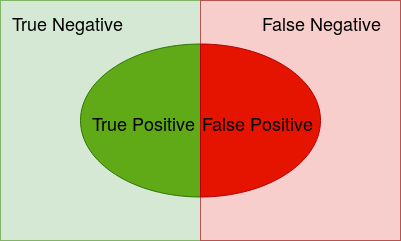
\includegraphics[width=100mm, keepaspectratio]{figures/F_score.png}
	\caption{The visual representation of the concept of true positive, true negative, false positive and false negative measures.}
	\label{fig:TP_TN_FP_FN}
\end{figure}


\[TP_{node==1} = number\ of\ correctly\ guessed\ node==1\]
\[TN_{node==1} = number\ of\ correctly\ guessed\ node \neq 1\]
\[FP_{node==1} = number\ of\ incorrectly\ guessed\ node==1\]
\[FN_{node==1} = number\ of\ incorrectly\ guessed\ node \neq 1\]

With these measures we can calculate the precision and recall. The precision tells us the ratio of correct guesses of the class out of every time the model predicted that class. The recall is the ratio of the correct guesses out of every instance that are actually in the class. The harmonic mean of the precision and recall is the F-score.

\[precision = \frac{TP}{TP + FN}\]
\[recall = \frac{TP}{TP + FP}\]

\[F1 = 2 * \frac{precision * recall}{precision + recall}\]

I constructed extractive summaries from the resulting graphs and the original articles multiple ways described in section~\ref{ssect:ExperimnetsAndResults} and calculated the various ROUGE scores for each method's output.

\section{Experiments and results}\label{ssect:ExperimnetsAndResults}
I have experimented with both the Encode Process Decode and the Graph Attention Network models with varying success.
\subsection{Encode Process Decode}
At first I tried to get the Encode-Process-Decode model to predict whether to put something in the summary graph or not using only the word ids as features, but realized it would probably be more sufficient to also use the POS tags.

I also experimented with different loss functions, but for now i decided to use softmax cross entropy with output feature sizes of 2.

Training on more, than 7000 articles for 5 epochs (Early stopping stopped it from running any longer) I've got the following results.

\[Softmax\ cross\ entropy\ loss\ on\ nodes\ and\ edges\ averaged = 0.447\]

The classification report on the test set. These nodes are the ones that were in the summary:

\begin{table}[!ht]
	\centering
	\begin{tabular}{| c | c |}
		\hline
		\textbf{precision on nodes}&62.8 \\ \hline
		\textbf{recall on nodes}&21.3 \\ \hline
		\textbf{F1 on nodes}&31.9 \\ \hline
	\end{tabular}
	\caption{Classification report on the nodes. The edges achieved 0 F1 scores}
\end{table}

As you can see from this the network hardly ever classifies a node as "1", meaning that it should be in the summary graph, but when it does it is 62.8\% accurate. This might be because the relative frequency of the "1" nodes is lower, than the "0" nodes' so the network predicts "0" nodes to be more likely.

This model has not been further evaluated.

\FloatBarrier

\subsection{SimpleGraphAttention Network}
I trained the network on the whole training set (80\% of the whole dataset) for 3 epochs. It stopped after the third epoch because of the early stopping mechanism.

I evaluated the trained network on the test set and the results are the following:

\[Softmax\ cross\ entropy\ loss\ on\ nodes = 0.809\]
The classification report on the test set. These nodes and edges are the ones that were in the summary:
\begin{table}[!ht]
	\centering
	\begin{tabular}{| c | c |}
		\hline
		\textbf{precision on nodes}&53.4 \\ \hline
		\textbf{recall on nodes}&54.2 \\ \hline
		\textbf{F1 on nodes}&53.8 \\ \hline
	\end{tabular}
	\caption{Classification report on the nodes.}
\end{table}

\subsubsection{Summary reconstruction and evaluation}
I tried three different approaches at the summary extraction, each have been evaluated by the ROUGE scoring mechanism. For this I used the perl based pyrouge package.

\paragraph{Reconstruction with the node average}

This reconstruction method scores each sentence of the original article using the equation below where the \(score_{word}\) is the predicted probability of the word (node) being in the summary graph.

\[score_{sentence} = \frac{\sum_{word \in sentence\ and\ word \notin stopwords} score_{word}}{|word \in sentence\ and\ word \notin stopwords|}\]

Based on the calculated score of each sentence we can order them by their relevance and keep the four most relevant sentences from the article as the summary.

This method does not utilize the information of the graph structure nor does it prefer longer sentences. As a result the average number of words in a summary is 75.97.

For fair comparison I generated shorter TextRank based gensim summaries and cut down the number of sentences in the extracted summaries. I did this by comparing the number of words in each reconstructed summary and chose the number of sentences so the word counts would be as close as possible in each pair.

\begin{table}[!ht]
	\centering
	\begin{tabular}{| l | c | c | c |}
		\hline
		\textbf{Evaluation method}&\textbf{System}&\textbf{Gensim}&\textbf{Maximum}\\ \hline \hline
		\textbf{average word count}&76&77&74 \\ \hline
		\textbf{ROUGE-1}&39.06&41.77&59.11 \\ \hline
		\textbf{ROUGE-2}&12.56&14.08&29.95 \\ \hline
		\textbf{ROUGE-L}&24.03&25.99&40.66 \\ \hline
		\textbf{ROUGE-SU*}&15.60&17.34&33.73 \\ \hline
	\end{tabular}
	\caption{ROUGE scores on the test set with reconstruction method using only the node scores}
	\label{tab:simple_node}
\end{table}
\FloatBarrier

\paragraph{Reconstruction with just the graph structure}

Contrary to the previous version this construction method does not use the output of the graph neural network but it is included here as contrast and as a step toward the next summarization method.

\begin{eqnarray*}
	score_{sentence} = \sum_{edge \in sentence\ graph} &[1\ if\ sender\ word \notin stopwords] + \\&[1\ if\ receiver\ word \notin stopwords]
\end{eqnarray*}

This score is basically the degree of each non-stopword node in a sentences summed. The ordering of sentences is based on this score. The summary contains the four best sentences. The average length of a summary is 138.42 word.

\begin{table}[!ht]
	\centering
	\begin{tabular}{| l | c | c | c |}
		\hline
		\textbf{Evaluation method}&\textbf{System}&\textbf{Gensim}&\textbf{Maximum}\\ \hline \hline
		
		\textbf{average word count}&138&136&104 \\ \hline
		\textbf{ROUGE-1}&54.17&56.35&73.91 \\ \hline
		\textbf{ROUGE-2}&18.82&20.80&39.29 \\ \hline
		\textbf{ROUGE-L}&32.68&34.47&51.01 \\ \hline
		\textbf{ROUGE-SU*}&26.69&29.27&49.15 \\ \hline
	\end{tabular}
	\caption{ROUGE scores on the test set with reconstruction method using just the graph structure}
	\label{tab:structure}
\end{table}
\FloatBarrier

\paragraph{Reconstruction with the graph structure and the node scores}

This method is the blend of the previous two. It utilizes the structure of the graph but also uses the output of the graph neural network.
\begin{eqnarray*}
	score_{sentence} = \sum_{edge \in sentence\ graph} &[score_{sender\ word}\ if\ sender\ word \notin stopwords] + \\&[score_{receiver\ word}\ if\ receiver\ word \notin stopwords]
\end{eqnarray*}
These summaries also contain the best four sentences. The average number of words in these summaries are 127.11.
\begin{table}[!ht]
	\centering
	\begin{tabular}{| l | c | c | c |}
		\hline
		\textbf{Evaluation method}&\textbf{System}&\textbf{Gensim}&\textbf{Maximum}\\ \hline \hline
		\textbf{average word count}&127&136&104 \\ \hline
		\textbf{ROUGE-1}&56.80&56.35&73.91 \\ \hline
		\textbf{ROUGE-2}&21.97&20.80&39.29 \\ \hline
		\textbf{ROUGE-L}&34.95&34.47&51.01 \\ \hline
		\textbf{ROUGE-SU*}&29.45&29.27&49.15 \\ \hline
	\end{tabular}
	\caption{ROUGE scores on the test set with reconstruction method using both graph structure and the node scores}
	\label{tab:simple_complete}
\end{table}

\subsubsection{Example}
To better visualize the results I compare the summary graph from Chapter~\ref{sect:DataProcessing} (Figure~\ref{fig:usain_summary_graph} and) to the calculated graph (Figure~\ref{fig:usain_bolt_predicted0}). The generated summaries are also written below.

\begin{figure}[!ht]
	\centering
	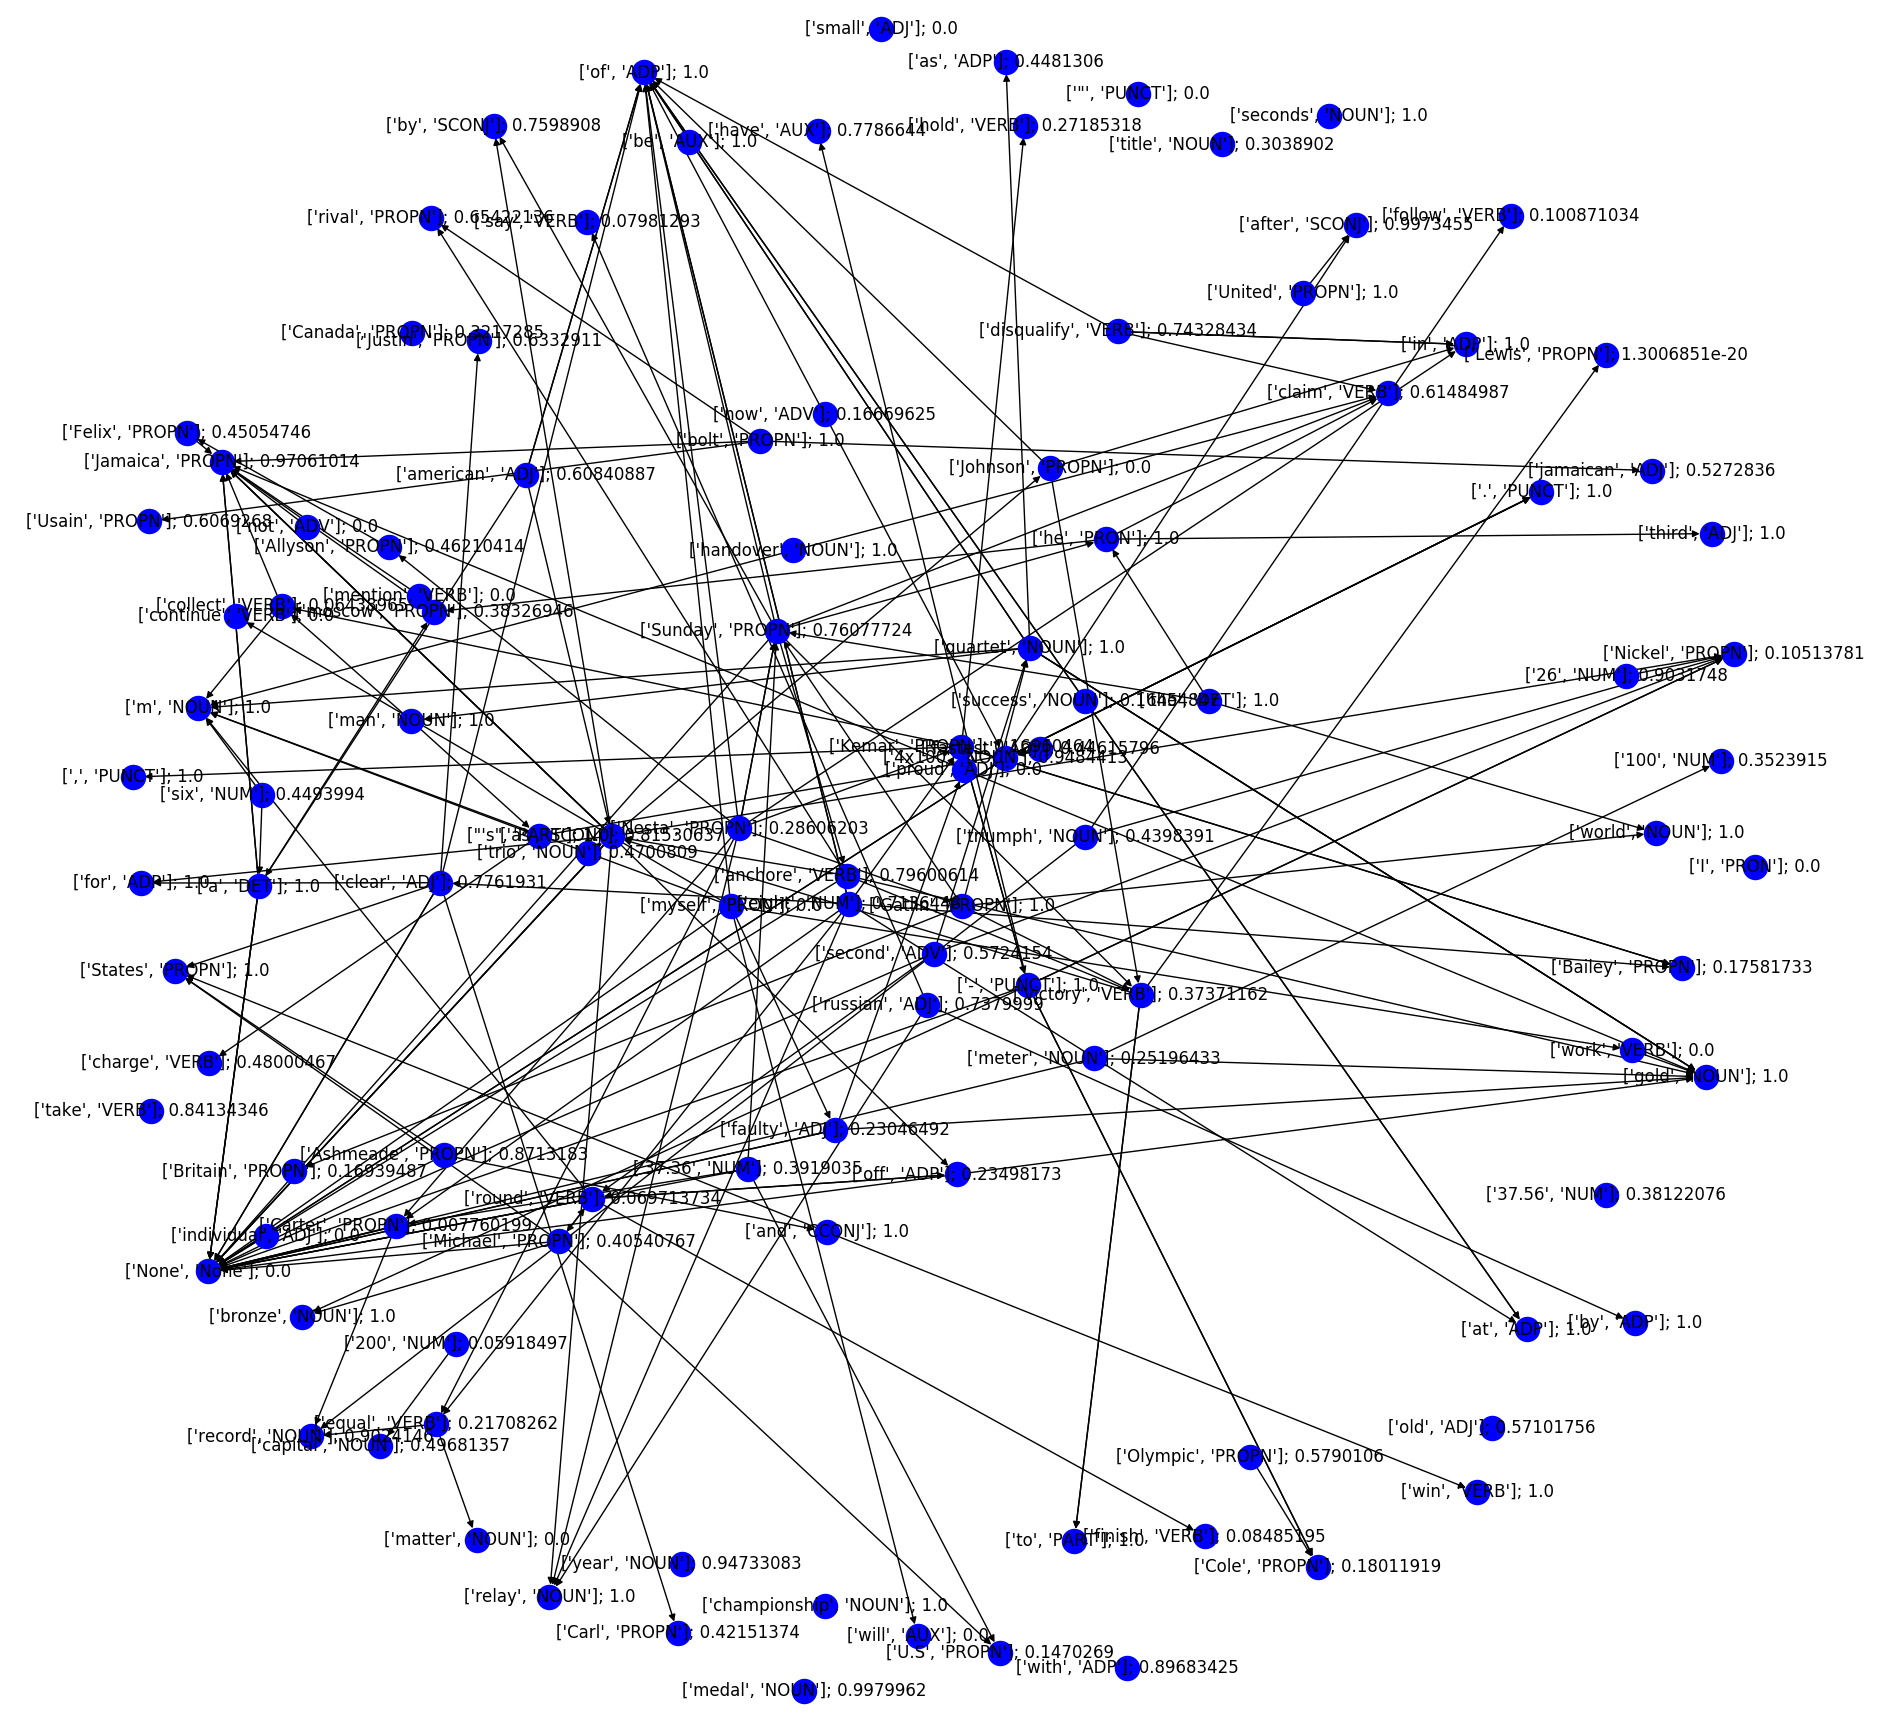
\includegraphics[width=150mm, keepaspectratio]{figures/usain_bolt_predicted.png}
	\caption{The calculated summary graph of the example article with just the nodes labeled 1.}
	\label{fig:usain_bolt_predicted0}
\end{figure}

\FloatBarrier

\textbox{
	\textbf{Reconstruction with the node average}
	
	Fraser-Pryce, like Bolt aged 26, became the first woman to achieve three golds in the 100-200 and the relay.
	Usain Bolt rounded off the world championships Sunday by claiming his third gold in Moscow as he anchored Jamaica to victory in the men's 4x100m relay.
	The British quartet, who were initially fourth, were promoted to the bronze which eluded their men's team.
	Bolt's final dash for golden glory brought the eight-day championship to a rousing finale, but while the hosts topped the medal table from the United States there was criticism of the poor attendances in the Luzhniki Stadium.
	
	\textbf{Reconstruction with just the graph structure}
	
	The 26-year-old Bolt has now collected eight gold medals at world championships, equaling the record held by American trio Carl Lewis, Michael Johnson and Allyson Felix, not to mention the small matter of six Olympic titles.
	Earlier, Jamaica's women underlined their dominance in the sprint events by winning the 4x100m relay gold, anchored by Shelly-Ann Fraser-Pryce, who like Bolt was completing a triple.
	The fastest man in the world charged clear of United States rival Justin Gatlin as the Jamaican quartet of Nesta Carter, Kemar Bailey-Cole, Nickel Ashmeade and Bolt won in 37.36 seconds.
	Defending champions, the United States, were initially back in the bronze medal position after losing time on the second handover between Alexandria Anderson and English Gardner, but promoted to silver when France were subsequently disqualified for an illegal handover.
	
	\textbf{Reconstruction with the graph structure and the node scores}
	
	The fastest man in the world charged clear of United States rival Justin Gatlin as the Jamaican quartet of Nesta Carter, Kemar Bailey-Cole, Nickel Ashmeade and Bolt won in 37.36 seconds.
	Defending champions, the United States, were initially back in the bronze medal position after losing time on the second handover between Alexandria Anderson and English Gardner, but promoted to silver when France were subsequently disqualified for an illegal handover.
	Germany's Christina Obergfoll finally took gold at global level in the women's javelin after five previous silvers, while Kenya's Asbel Kiprop easily won a tactical men's 1500m final.
	Earlier, Jamaica's women underlined their dominance in the sprint events by winning the 4x100m relay gold, anchored by Shelly-Ann Fraser-Pryce, who like Bolt was completing a triple.}{
	\caption{Example article summaries}}

\subsection{GraphAttention Network}

I trained this model on ten-thousand data for 3 epochs. In each epoch the network trained on different data, all in all I used thirty-thousand input and target output. It stopped after the third epoch because of the early stopping mechanism.

Due to time constraints I was unable to train the network on the whole training data.

I evaluated the trained network and the results are the following:

\[Softmax\ cross\ entropy\ loss\ on\ nodes = 0.7996\]
The classification report on the test set. These nodes and edges are the ones that were in the summary:

\begin{table}[!ht]
	\centering
	\begin{tabular}{| c | c |}
		\hline
		\textbf{precision on nodes}&43.1 \\ \hline
		\textbf{recall on nodes}&63.8 \\ \hline
		\textbf{F1 on nodes}&51.4 \\ \hline
	\end{tabular}
	\caption{Classification report on the nodes.}
\end{table}

\subsubsection{Summary reconstruction and evaluation}
I tried the same reconstruction method for the results of the GraphAttention model. Keep in mind that this model has been trained for less time and on less data.

\paragraph{Reconstruction with the node average}

The average number of words in a four sentence long summary is 75.65.

\begin{table}[!ht]
	\centering
	\begin{tabular}{| l | c | c | c |}
	\hline
	\textbf{Evaluation method}&\textbf{System}&\textbf{Gensim}&\textbf{Maximum}\\ \hline \hline
	\textbf{average word count}&76&77&74 \\ \hline
	\textbf{ROUGE-1}&36.27&41.77&59.11 \\ \hline
	\textbf{ROUGE-2}&11.25&14.08&29.95 \\ \hline
	\textbf{ROUGE-L}&22.55&25.99&40.66 \\ \hline
	\textbf{ROUGE-SU*}&14.22&17.34&33.73 \\ \hline
	\end{tabular}
	\caption{ROUGE scores on the test set with reconstruction method using only the node scores}
	\label{tab:attended_node}
\end{table}

\paragraph{Reconstruction with just the graph structure}

The result is the same as before, since we only consider the graph structures and they haven't changed.

\paragraph{Reconstruction with the graph structure and the node scores}

The average word count in a four sentence long summary is 130.21.

\begin{table}[!ht]
	\centering
	\begin{tabular}{| l | c | c | c |}
	\hline
		\textbf{Evaluation method}&\textbf{System}&\textbf{Gensim}&\textbf{Maximum}\\ \hline \hline
		\textbf{average word count}&130&136&104 \\ \hline
		\textbf{ROUGE-1}&51.14&56.35&73.91 \\ \hline
		\textbf{ROUGE-2}&18.02&20.80&39.29 \\ \hline
		\textbf{ROUGE-L}&31.41&34.47&51.01 \\ \hline
		\textbf{ROUGE-SU*}&25.19&29.27&49.15 \\ \hline
	\end{tabular}
	\caption{ROUGE scores on the test set with reconstruction method using both graph structure and the node scores}
	\label{tab:attended_complete}
\end{table}

\subsubsection{Example}
Similarly to the previous case I compared the summary graph from Chapter~\ref{sect:DataProcessing} (Figure~\ref{fig:usain_summary_graph} and) to the calculated graph (Figure~\ref{fig:usain_bolt_predicted1}). The generated summaries are also written below.

\begin{figure}[!ht]
	\centering
	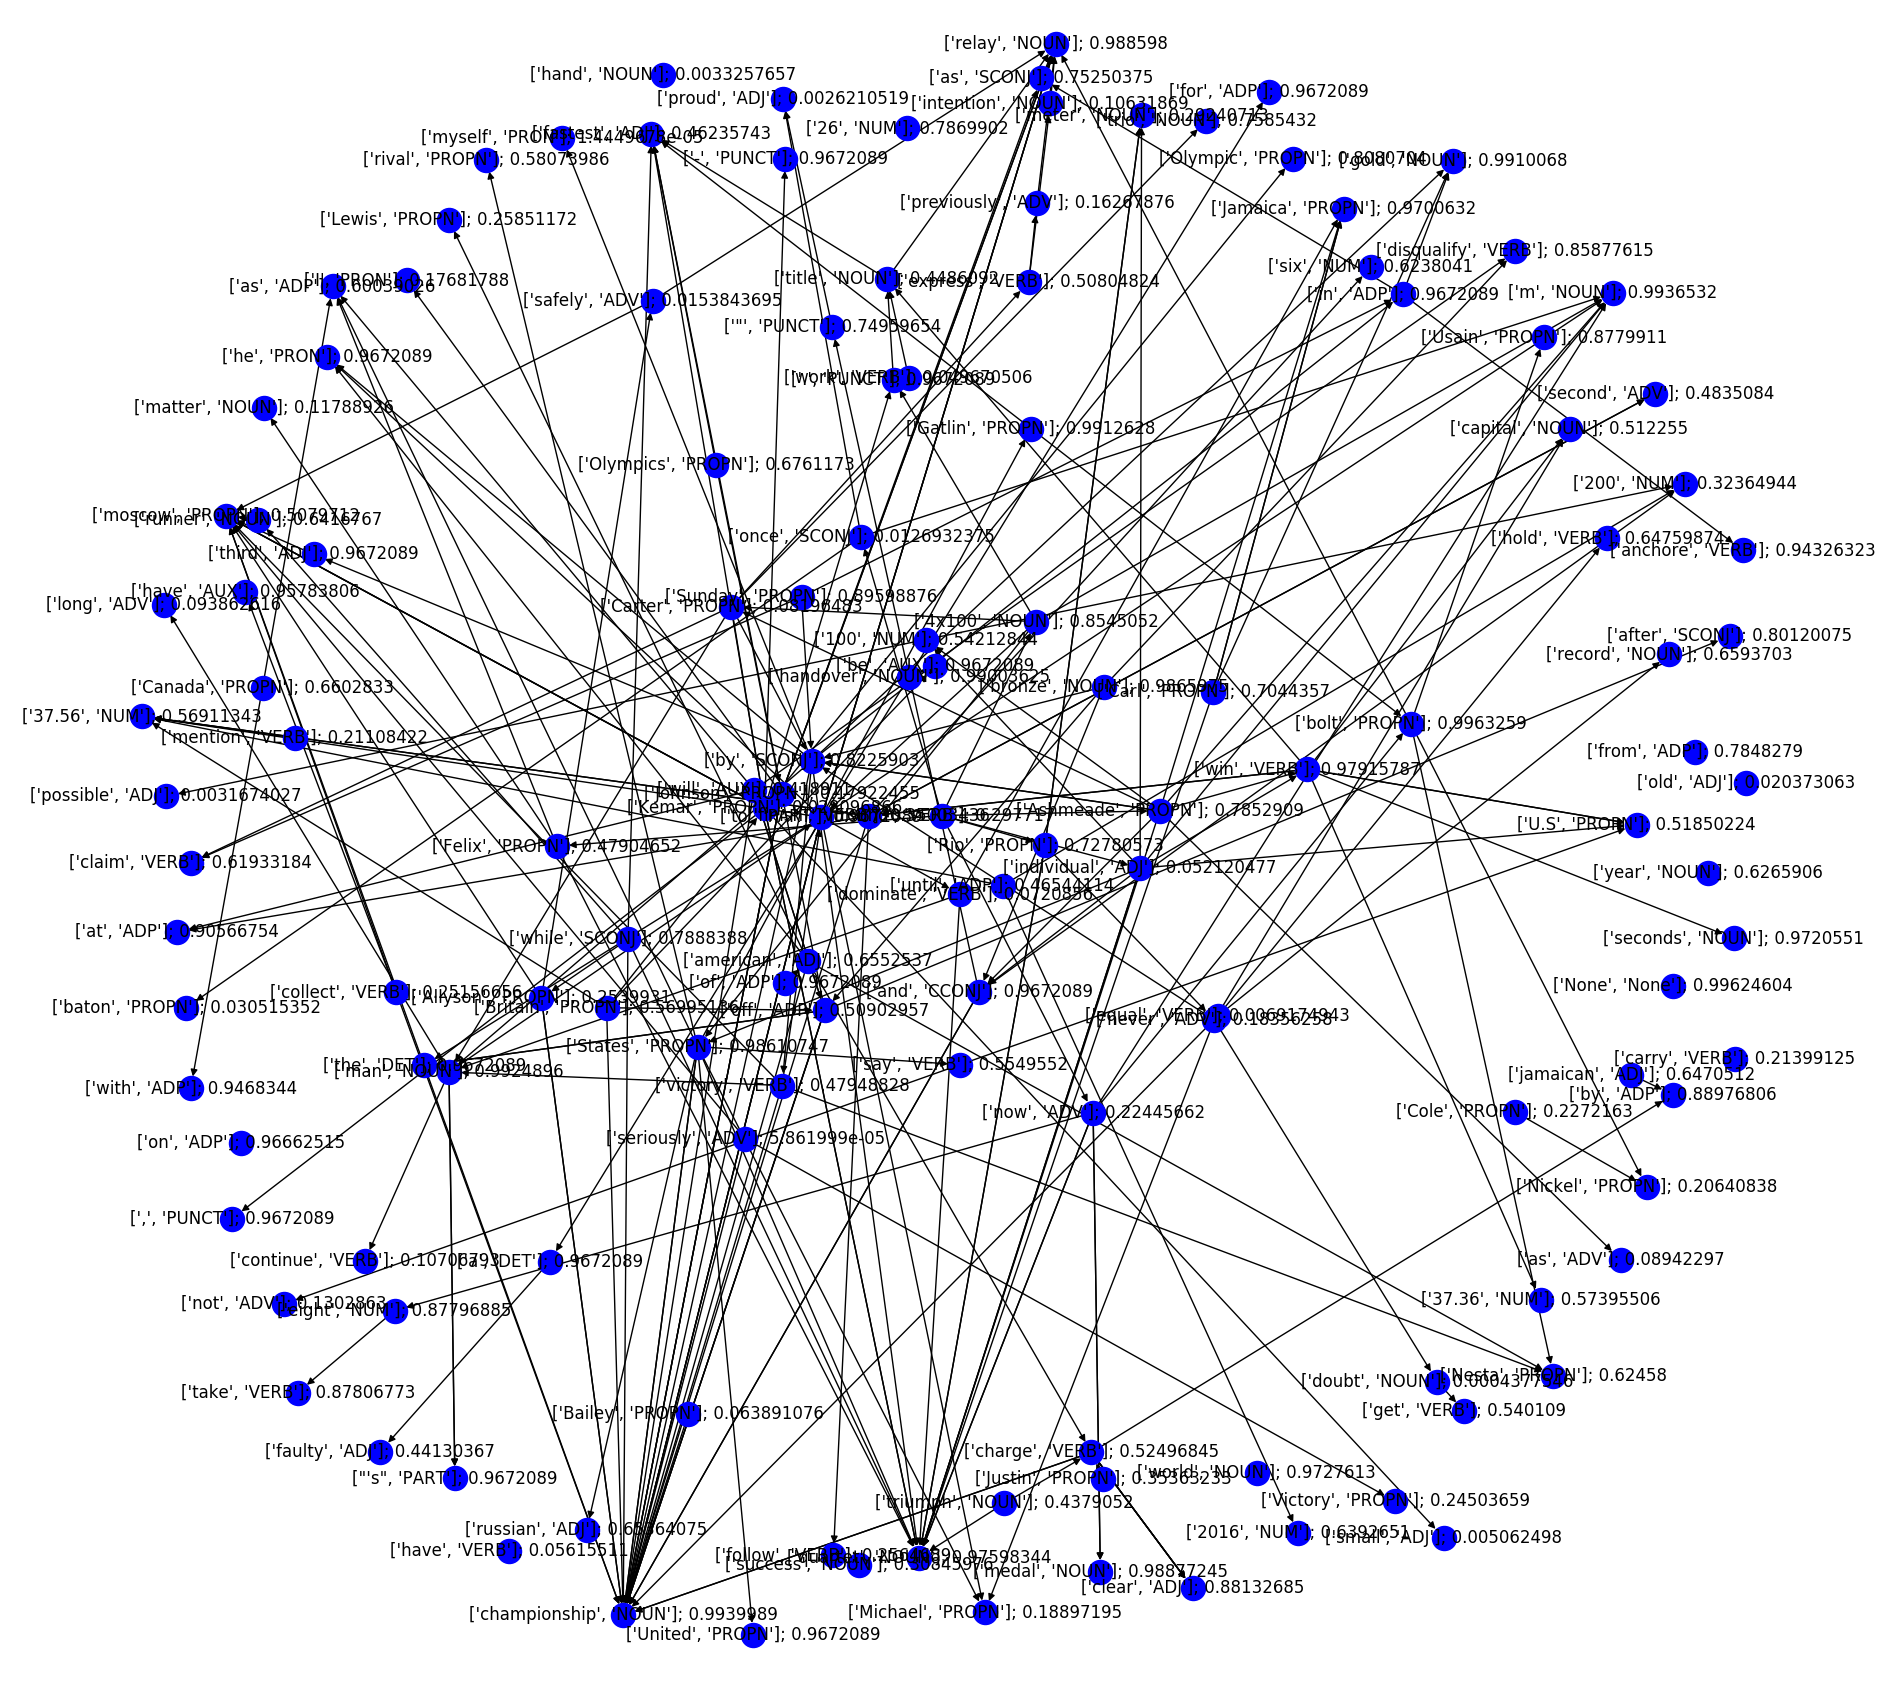
\includegraphics[width=150mm, keepaspectratio]{figures/usain_bolt_predicted_attended.png}
	\caption{The calculated summary graph of the example article with just the nodes labeled 1.}
	\label{fig:usain_bolt_predicted1}
\end{figure}

\FloatBarrier

\textbox{
	\textbf{Reconstruction with the node average}
	
	Usain Bolt rounded off the world championships Sunday by claiming his third gold in Moscow as he anchored Jamaica to victory in the men's 4x100m relay.
	Fraser-Pryce, like Bolt aged 26, became the first woman to achieve three golds in the 100-200 and the relay.
	The British quartet, who were initially fourth, were promoted to the bronze which eluded their men's team.
	The U.S finished second in 37.56 seconds with Canada taking the bronze after Britain were disqualified for a faulty handover.
	
	\textbf{Reconstruction with the graph structure and the node scores}
	
	The fastest man in the world charged clear of United States rival Justin Gatlin as the Jamaican quartet of Nesta Carter, Kemar Bailey-Cole, Nickel Ashmeade and Bolt won in 37.36 seconds.
	Defending champions, the United States, were initially back in the bronze medal position after losing time on the second handover between Alexandria Anderson and English Gardner, but promoted to silver when France were subsequently disqualified for an illegal handover.
	Earlier, Jamaica's women underlined their dominance in the sprint events by winning the 4x100m relay gold, anchored by Shelly-Ann Fraser-Pryce, who like Bolt was completing a triple.
	Germany's Christina Obergfoll finally took gold at global level in the women's javelin after five previous silvers, while Kenya's Asbel Kiprop easily won a tactical men's 1500m final.}{}
\FloatBarrier

\section{Comparison between models}

Table~\ref{tab:short} contains the comparable ROUGE scores of the SimpleGraphAttention model's and the GraphAttention model's summaries reconstructed with the node average method and also the TextRank based benchmark method's output followed by the maximum achievable ROUGE scores with the adequate summary lengths. These data is directly from table~\ref{tab:simple_node} and table~\ref{tab:attended_node}.

\begin{table}[!ht]
	\centering
	\begin{tabular}{| l | c | c | c | c |}
		\hline
		\textbf{Metric}&\textbf{Simple node avg}&\textbf{Attended node avg}&\textbf{TextRank}&\textbf{Maximum} \\ \hline \hline
		\textbf{avg words}&76&76&77&74 \\ \hline
		\textbf{ROUGE-1}&39.06&36.27&41.77&59.11 \\ \hline
		\textbf{ROUGE-2}&12.56&11.25&14.08&29.95 \\ \hline
		\textbf{ROUGE-L}&24.03&22.55&25.99&40.66 \\ \hline
		\textbf{ROUGE-SU*}&15.60&14.22&17.34&33.73 \\ \hline
	\end{tabular}
	\caption{Short summary comparisons. \\ The \textbf{Simple node avg} is the graph generated with the SimpleGraphAttention model and the summary constructed by the node averaging method. \\ The \textbf{Attended node avg} is the graph generated with the GraphAttention model and the summary constructed by the node averaging method. \\ The \textbf{TextRank} is the summary generated with gensim's TextRank method. \\ The \textbf{Maximum} is the highest achievable ROUGE score with the similar length.}
	\label{tab:short}
\end{table}

Table~\ref{tab:long} contains the comparable ROUGE scores of the SimpleGraphAttention model's and the GraphAttention model's summaries reconstructed with the node scores and the graph structure and also the TextRank based benchmark method's output followed by the maximum achievable ROUGE scores all constructed by the top 4 sentences. These data is directly from table~\ref{tab:structure}, table~\ref{tab:simple_complete} and table~\ref{tab:attended_complete}.

\begin{table}[!ht]
	\centering
	\begin{tabular}{| l | c | c | c | c | c |}
		\hline
		\textbf{Metric}&\textbf{Just structure}&\textbf{Simple}&\textbf{Attended}&\textbf{TextRank}&\textbf{Maximum} \\ \hline \hline
		\textbf{avg words}&138&127&130&136&104 \\ \hline
		\textbf{ROUGE-1}&54.17&56.80&51.14&56.35&73.91 \\ \hline
		\textbf{ROUGE-2}&18.82&21.97&18.02&20.80&39.29 \\ \hline
		\textbf{ROUGE-L}&32.68&34.95&31.42&34.47&51.01 \\ \hline
		\textbf{ROUGE-SU*}&26.69&29.45&25.19&29.27&49.15 \\ \hline
	\end{tabular}
	\caption{Long summary comparisons \\ The \textbf{Just structure} is the summary constructed by the node's degree. \\ The \textbf{Simple} is the graph generated with the SimpleGraphAttention model and the summary constructed by the method that takes into account the graph structure and the node score as well. \\ The \textbf{Attended} is the graph generated with the GraphAttention model and the summary constructed by the method that takes into account the graph structure and the node score as well. \\ The \textbf{TextRank} is the summary generated with gensim's TextRank method. \\ The \textbf{Maximum} is the highest achievable ROUGE score with the similar length.}
	\label{tab:long}
\end{table}

\FloatBarrier
\subsection{Results by summary length}

\begin{figure}[!ht]
	\centering
	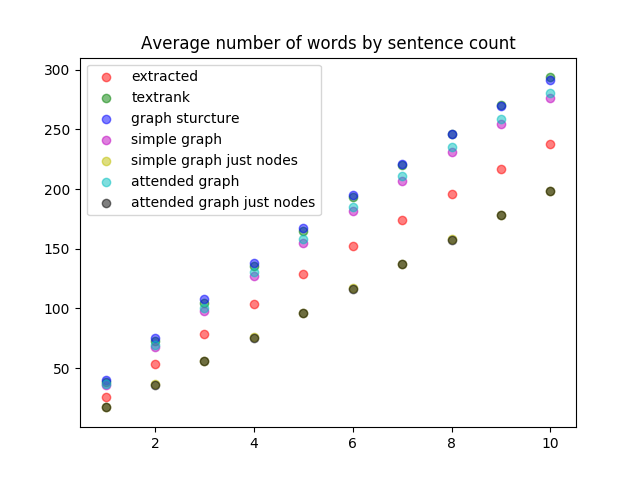
\includegraphics[width=150mm, keepaspectratio]{figures/word_counts.png}
	\caption{The average number of words by the number of sentences in the summary.}
	\label{fig:word_count}
\end{figure}

\begin{table}[!ht]
	\centering
	\begin{tabular}{| l | c | c | c | c | c | c | c | c | c | c |}
		\hline
		\textbf{Model/Length}&\textbf{1}&\textbf{2}&\textbf{3}&\textbf{4}&\textbf{5}&\textbf{6}&\textbf{7}&\textbf{8}&\textbf{9}&\textbf{10} \\ \hline \hline
		\textbf{Maximum}&26&53&79&104&129&152&174&196&217&238 \\ \hline
		\textbf{TextRank}&39&73&105&136&165&193&220&246&271&294 \\ \hline
		\textbf{G. struct}&40&75&108&138&167&195&221&246&269&292 \\ \hline
		\textbf{S. graph}&36&68&98&127&155&182&207&231&255&277 \\ \hline
		\textbf{S. node}&17&36&56&76&96&117&137&158&178&199 \\ \hline
		\textbf{A. graph}&37&70&101&130&158&185&211&235&258&281 \\ \hline
		\textbf{A. node}&17&36&56&76&96&116&137&157&178&198 \\ \hline
	\end{tabular}
	\caption{The average word counts by the number of sentences in the summary
		\\ The \textbf{Maximum} is the summary created by the greedy algorithm.
		\\ The \textbf{TextRank} is the summary generated with gensim's TextRank method. 
		\\The \textbf{G. struct} is the summary constructed by the node's degree.
		\\ The \textbf{S. graph} is the graph generated with the SimpleGraphAttention model and the summary constructed by the method that takes into account the graph structure and the node score as well.
		\\ The \textbf{S. node} is the graph generated with the SimpleGraphAttention model and the summary constructed by the node averaging method.
		\\ The \textbf{A. graph} is the graph generated with the GraphAttention model and the summary constructed by the method that takes into account the graph structure and the node score as well.
		 \\ The \textbf{A. node} is the graph generated with the GraphAttention model and the summary constructed by the node averaging method.}
	\label{tab:word_count}
\end{table}

\FloatBarrier

\begin{figure}[!ht]
	\centering
	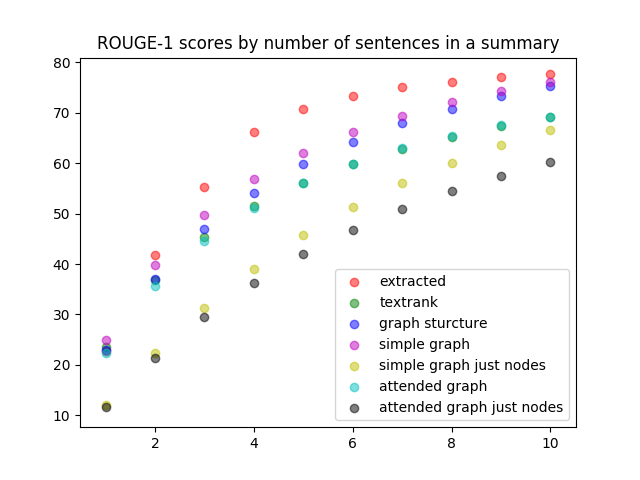
\includegraphics[width=150mm, keepaspectratio]{figures/ROUGE_1.png}
	\caption{The ROUGE-1 score  by the number of sentences in the summary.}
	\label{fig:ROUGE-1}
\end{figure}

\begin{table}[!ht]
	\centering
	\begin{tabular}{| l | c | c | c | c | c | c | c | c | c | c |}
		\hline
		\textbf{M/L}&\textbf{1}&\textbf{2}&\textbf{3}&\textbf{4}&\textbf{5}&\textbf{6}&\textbf{7}&\textbf{8}&\textbf{9}&\textbf{10} \\ \hline \hline
		\textbf{Maximum}&22.75&41.72&55.34&66.24&70.85&73.42&75.07&76.22&77.03&77.63 \\ \hline
		\textbf{Textrank}&23.58&36.83&45.4&51.51&56.15&59.82&62.8&65.26&67.37&69.14 \\ \hline
		\textbf{G. struct}&22.93&37.05&46.9&54.19&59.85&64.31&67.92&70.85&73.3&75.35 \\ \hline
		\textbf{S. graph}&24.88&39.77&49.74&56.79&62.08&66.18&69.47&72.1&74.29&76.11 \\ \hline
		\textbf{S. node}&11.95&22.38&31.33&39.06&45.69&51.34&56.1&60.12&63.55&66.53 \\ \hline
		\textbf{A. graph}&22.28&35.66&44.66&51.14&56.08&59.91&62.99&65.49&67.53&69.27 \\ \hline
		\textbf{A. node}&11.54&21.34&29.47&36.27&41.93&46.76&50.92&54.47&57.55&60.18 \\ \hline
	\end{tabular}
	\caption{The ROUGE-1 score by the number of sentences in the summary
		\\ The \textbf{Maximum} is the summary created by the greedy algorithm.
		\\ The \textbf{TextRank} is the summary generated with gensim's TextRank method. 
		\\The \textbf{G. struct} is the summary constructed by the node's degree.
		\\ The \textbf{S. graph} is the graph generated with the SimpleGraphAttention model and the summary constructed by the method that takes into account the graph structure and the node score as well.
		\\ The \textbf{S. node} is the graph generated with the SimpleGraphAttention model and the summary constructed by the node averaging method.
		\\ The \textbf{A. graph} is the graph generated with the GraphAttention model and the summary constructed by the method that takes into account the graph structure and the node score as well.
		\\ The \textbf{A. node} is the graph generated with the GraphAttention model and the summary constructed by the node averaging method.}
	\label{tab:ROUGE-1}
\end{table}

\FloatBarrier

\begin{figure}[!ht]
	\centering
	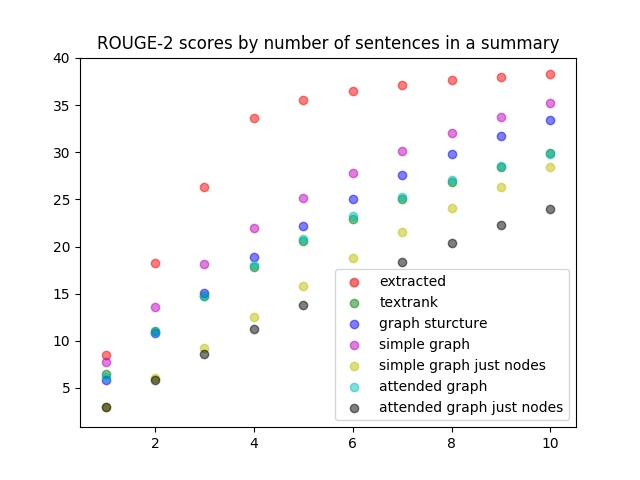
\includegraphics[width=150mm, keepaspectratio]{figures/ROUGE_2.png}
	\caption{The ROUGE-2 score  by the number of sentences in the summary.}
	\label{fig:ROUGE-2}
\end{figure}

\begin{table}[!ht]
	\centering
	\begin{tabular}{| l | c | c | c | c | c | c | c | c | c | c |}
		\hline
		\textbf{M/L}&\textbf{1}&\textbf{2}&\textbf{3}&\textbf{4}&\textbf{5}&\textbf{6}&\textbf{7}&\textbf{8}&\textbf{9}&\textbf{10} \\ \hline \hline
		\textbf{Maximum}&8.5&18.25&26.33&33.65&35.52&36.51&37.16&37.62&37.97&38.25 \\ \hline
		\textbf{Textrank}&6.47&11.07&14.75&17.88&20.58&22.94&25.01&26.83&28.46&29.9 \\ \hline
		\textbf{G. struct}&5.84&10.79&15.1&18.84&22.15&25.04&27.56&29.77&31.72&33.45 \\ \hline
		\textbf{S. graph}&7.77&13.54&18.18&21.97&25.13&27.8&30.1&32.04&33.73&35.23 \\ \hline
		\textbf{S. node}&2.95&6.04&9.28&12.56&15.78&18.79&21.54&24.04&26.31&28.38 \\ \hline
		\textbf{A. graph}&6.17&10.9&14.76&18.02&20.79&23.19&25.25&27.01&28.52&29.85 \\ \hline
		\textbf{A. node}&2.93&5.8&8.58&11.25&13.77&16.15&18.38&20.41&22.3&23.98 \\ \hline
	\end{tabular}
	\caption{The ROUGE-2 score by the number of sentences in the summary
		\\ The \textbf{Maximum} is the summary created by the greedy algorithm.
		\\ The \textbf{TextRank} is the summary generated with gensim's TextRank method. 
		\\The \textbf{G. struct} is the summary constructed by the node's degree.
		\\ The \textbf{S. graph} is the graph generated with the SimpleGraphAttention model and the summary constructed by the method that takes into account the graph structure and the node score as well.
		\\ The \textbf{S. node} is the graph generated with the SimpleGraphAttention model and the summary constructed by the node averaging method.
		\\ The \textbf{A. graph} is the graph generated with the GraphAttention model and the summary constructed by the method that takes into account the graph structure and the node score as well.
		\\ The \textbf{A. node} is the graph generated with the GraphAttention model and the summary constructed by the node averaging method.}
	\label{tab:ROUGE-2}
\end{table}

\FloatBarrier

\begin{figure}[!ht]
	\centering
	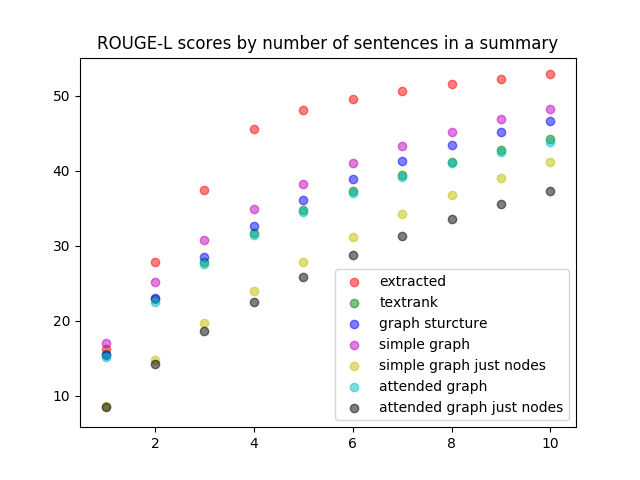
\includegraphics[width=150mm, keepaspectratio]{figures/ROUGE_L.png}
	\caption{The ROUGE-L score  by the number of sentences in the summary.}
	\label{fig:ROUGE-L}
\end{figure}

\begin{table}[!ht]
	\centering
	\begin{tabular}{| l | c | c | c | c | c | c | c | c | c | c |}
		\hline
		\textbf{M/L}&\textbf{1}&\textbf{2}&\textbf{3}&\textbf{4}&\textbf{5}&\textbf{6}&\textbf{7}&\textbf{8}&\textbf{9}&\textbf{10} \\ \hline \hline
		\textbf{Maximum}&16.26&27.88&37.43&45.58&48.09&49.6&50.7&51.55&52.27&52.87 \\ \hline
		\textbf{Textrank}&15.65&22.89&27.88&31.66&34.75&37.3&39.44&41.26&42.84&44.21 \\ \hline
		\textbf{G. struct}&15.42&23.05&28.47&32.69&36.14&38.98&41.39&43.45&45.21&46.73 \\ \hline
		\textbf{S. graph}&17.09&25.16&30.74&34.95&38.31&41.05&43.36&45.26&46.89&48.29 \\ \hline
		\textbf{S. node}&8.69&14.73&19.7&24.03&27.87&31.26&34.23&36.83&39.12&41.21 \\ \hline
		\textbf{A. graph}&15.21&22.48&27.54&31.42&34.5&37.06&39.22&41.02&42.55&43.87 \\ \hline
		\textbf{A. node}&8.46&14.2&18.72&22.55&25.84&28.74&31.31&33.58&35.6&37.39 \\ \hline
	\end{tabular}
	\caption{The ROUGE-L score by the number of sentences in the summary
		\\ The \textbf{Maximum} is the summary created by the greedy algorithm.
		\\ The \textbf{TextRank} is the summary generated with gensim's TextRank method. 
		\\The \textbf{G. struct} is the summary constructed by the node's degree.
		\\ The \textbf{S. graph} is the graph generated with the SimpleGraphAttention model and the summary constructed by the method that takes into account the graph structure and the node score as well.
		\\ The \textbf{S. node} is the graph generated with the SimpleGraphAttention model and the summary constructed by the node averaging method.
		\\ The \textbf{A. graph} is the graph generated with the GraphAttention model and the summary constructed by the method that takes into account the graph structure and the node score as well.
		\\ The \textbf{A. node} is the graph generated with the GraphAttention model and the summary constructed by the node averaging method.}
	\label{tab:ROUGE-L}
\end{table}

\FloatBarrier

\begin{figure}[!ht]
	\centering
	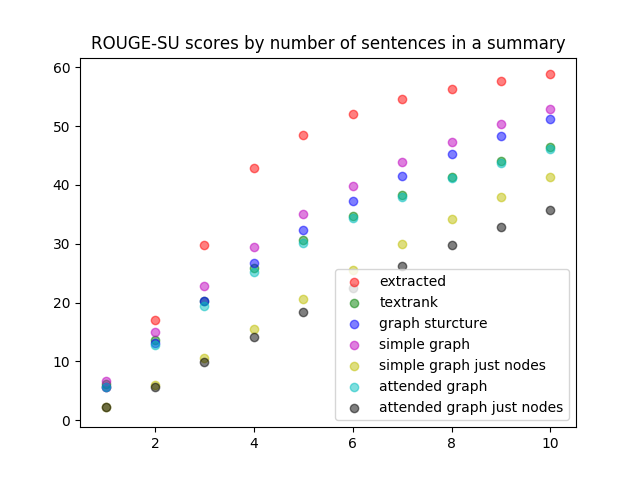
\includegraphics[width=150mm, keepaspectratio]{figures/ROUGE_SU.png}
	\caption{The ROUGE-SU* score  by the number of sentences in the summary.}
	\label{fig:ROUGE-SU}
\end{figure}

\begin{table}[!ht]
	\centering
	\begin{tabular}{| l | c | c | c | c | c | c | c | c | c | c |}
		\hline
		\textbf{M/L}&\textbf{1}&\textbf{2}&\textbf{3}&\textbf{4}&\textbf{5}&\textbf{6}&\textbf{7}&\textbf{8}&\textbf{9}&\textbf{10} \\ \hline \hline
		\textbf{Maximum}&5.71&17.06&29.77&42.81&48.57&52.12&54.58&56.39&57.74&58.79 \\ \hline
		\textbf{Textrank}&6.14&13.6&20.21&25.84&30.63&34.74&38.28&41.35&44.04&46.37 \\ \hline
		\textbf{G. struct}&5.75&13.2&20.32&26.71&32.36&37.25&41.51&45.19&48.4&51.2 \\ \hline
		\textbf{S. graph}&6.68&15.09&22.83&29.45&35.05&39.81&43.88&47.32&50.28&52.85 \\ \hline
		\textbf{S. node}&2.23&6.01&10.62&15.6&20.63&25.5&30.01&34.13&37.89&41.33 \\ \hline
		\textbf{A. graph}&5.65&12.79&19.42&25.19&30.16&34.39&38.03&41.14&43.79&46.11 \\ \hline
		\textbf{A. node}&2.2&5.75&9.89&14.22&18.42&22.45&26.24&29.72&32.93&35.81 \\ \hline
	\end{tabular}
	\caption{The ROUGE-SU* score by the number of sentences in the summary
		\\ The \textbf{Maximum} is the summary created by the greedy algorithm.
		\\ The \textbf{TextRank} is the summary generated with gensim's TextRank method. 
		\\The \textbf{G. struct} is the summary constructed by the node's degree.
		\\ The \textbf{S. graph} is the graph generated with the SimpleGraphAttention model and the summary constructed by the method that takes into account the graph structure and the node score as well.
		\\ The \textbf{S. node} is the graph generated with the SimpleGraphAttention model and the summary constructed by the node averaging method.
		\\ The \textbf{A. graph} is the graph generated with the GraphAttention model and the summary constructed by the method that takes into account the graph structure and the node score as well.
		\\ The \textbf{A. node} is the graph generated with the GraphAttention model and the summary constructed by the node averaging method.}
	\label{tab:ROUGE-SU}
\end{table}
